\section{Phương pháp}
\label{sec:method}

\subsection{Kiến trúc tổng thể}

Hệ thống gồm ba khối độc lập, ghép nối qua giao diện thống nhất (Hình~\ref{fig:pipeline}):

\begin{enumerate}
  \item \textbf{Retriever} $R$: với câu hỏi $q$, trả về top-$k$ đoạn văn từ kho $\mathcal{C}$.
  \item \textbf{Compressor} $C$: biến $(q, D)$ thành ngữ cảnh $c$ ngắn hơn. Mọi bộ nén đều trả về
  \emph{văn bản}, nên dùng được với bất kỳ LLM nào (kể cả qua API).
  \item \textbf{Generator}: LLM sinh câu trả lời từ prompt chuẩn của \citet{liu2024lost}.
\end{enumerate}

\begin{figure}[t]
\centering
\IfFileExists{figures/pipeline.pdf}{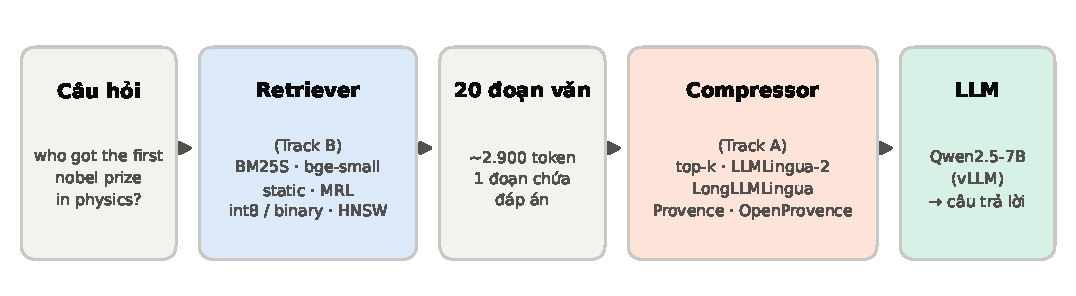
\includegraphics[width=\linewidth]{pipeline.pdf}}{\fbox{pipeline}}
\caption{Pipeline Efficient RAG: truy hồi $\rightarrow$ nén ngữ cảnh $\rightarrow$ sinh câu trả lời.
Track A đánh giá khối nén (với 20 đoạn cho sẵn), Track B đánh giá khối truy hồi.}
\label{fig:pipeline}
\end{figure}

\subsection{Các phương pháp nén ngữ cảnh}
\label{sec:compressors}

Chúng tôi chia các bộ nén thành bốn nhóm theo đơn vị bị loại bỏ (Bảng~\ref{tab:compressors}).

\paragraph{Tham chiếu.} \emph{Closed-book} (không ngữ cảnh) là cận dưới; \emph{Oracle} (chỉ đoạn vàng)
là cận trên thực tế; \emph{Full} (giữ nguyên 20 đoạn) là baseline cần vượt qua.

\paragraph{Mức prompt -- Truncate.} Giữ $B$ token đầu tiên của ngữ cảnh đầy đủ. Đây là cách ``ngây thơ''
nhất để đạt một ngân sách token; nó loại bỏ hoàn toàn các đoạn ở cuối.

\paragraph{Mức tài liệu -- Top-$k$ selection.} Chấm điểm từng đoạn theo câu hỏi rồi giữ $k$ đoạn có
điểm cao nhất, \emph{giữ nguyên thứ tự ban đầu}. Ba bộ chấm điểm: BM25 (thưa, từ vựng), bi-encoder
\texttt{bge-small-en-v1.5}~\cite{xiao2024cpack} (cosine), và cross-encoder \texttt{ms-marco-MiniLM-L6-v2}
(reranker). Với 20 đoạn trung bình $\sim$2.900 token, $k=10$ và $k=5$ tương ứng nén khoảng 2$\times$ và
4$\times$, khớp với hai mức ngân sách trong bảng của LongLLMLingua.

\paragraph{Mức token.} \textbf{LLMLingua-2}~\cite{pan2024llmlingua2}: bộ phân loại token
XLM-RoBERTa-large dự đoán xác suất giữ $p(\text{keep}\mid x_i)$; giữ các token có xác suất cao nhất
sao cho đạt tỉ lệ $r$ (ngưỡng toàn cục trên cả 20 đoạn). \textbf{LongLLMLingua}~\cite{jiang2024longllmlingua}:
tính perplexity có điều kiện câu hỏi bằng LM nhân quả nhỏ (Qwen2.5-0.5B-Instruct thay cho Llama-2-7B
trong bài gốc) để xếp hạng đoạn và nén token với ngân sách $B$ token. Ngoài ra, chúng tôi ghép
\textbf{reranker top-10 $\rightarrow$ LLMLingua-2 ($r=0{,}5$)} để mô phỏng chiến lược coarse-to-fine.

\paragraph{Mức câu -- Context pruning.} \textbf{Provence}~\cite{chirkova2025provence} là một cross-encoder
DeBERTa-v3-large với hai đầu ra: điểm liên quan của cả đoạn (reranking) và xác suất giữ của từng token,
được gộp thành quyết định giữ/bỏ từng \emph{câu} theo ngưỡng $\tau$. Ngưỡng nhỏ giữ nhiều câu hơn.
Đoạn không còn câu nào bị loại hẳn. \textbf{OpenProvence}~\cite{openprovence} dùng cùng ý tưởng với
backbone ModernBERT-base (150M tham số, nhỏ hơn 3 lần). Chúng tôi quét $\tau\in\{0{,}01; 0{,}1; 0{,}5\}$
cho Provence và $\tau\in\{0{,}1; 0{,}5\}$ cho OpenProvence.

\begin{table}[t]
\centering
\caption{Các bộ nén được đánh giá. ``Hỏi'' = có dùng câu hỏi khi nén.}
\label{tab:compressors}
\small
\begin{tabular}{l l l c r}
\toprule
Nhóm & Phương pháp & Mô hình & Hỏi & Tham số \\
\midrule
Tham chiếu & Closed-book / Oracle / Full & -- & -- & -- \\
Prompt & Truncate & -- & -- & 0 \\
Tài liệu & BM25 top-$k$ & BM25S & \checkmark & 0 \\
 & Dense top-$k$ & bge-small-en-v1.5 & \checkmark & 33M \\
 & Rerank top-$k$ & ms-marco-MiniLM-L6-v2 & \checkmark & 23M \\
Token & LLMLingua-2 & xlm-roberta-large & -- & 559M \\
 & LongLLMLingua & Qwen2.5-0.5B-Instruct & \checkmark & 494M \\
 & Rerank $\rightarrow$ LLMLingua-2 & MiniLM + XLM-R & \checkmark & 582M \\
Câu & Provence & deberta-v3-large & \checkmark & 435M \\
 & OpenProvence & gte-modernbert-base & \checkmark & 150M \\
\bottomrule
\end{tabular}
\end{table}

\paragraph{Tính bất biến theo thứ tự.} Các bộ nén mức tài liệu, mức câu và LLMLingua-2 xử lý từng đoạn
độc lập với vị trí của nó. Chúng tôi tận dụng tính chất này: kết quả nén của một tập đoạn được ghi nhớ
và tái sử dụng cho năm vị trí đoạn vàng (chỉ thứ tự thay đổi), giảm 5 lần thời gian nén; độ trễ báo cáo
là độ trễ đo ở lần tính đầu tiên. Sau khi nén, các đoạn còn lại \emph{giữ nguyên thứ tự} và được đánh
số lại, nhờ đó biến ``vị trí đoạn vàng'' vẫn có ý nghĩa, giống thiết lập của các bảng đã công bố.

\subsection{Các phương pháp truy hồi hiệu quả}

Trên kho gộp $\sim$50,7 nghìn đoạn, chúng tôi so sánh:
\begin{itemize}
  \item \textbf{BM25S}~\cite{lu2024bm25s} với stemming và loại stopword.
  \item \textbf{Static embedding} \texttt{static-retrieval-mrl-en-v1}~\cite{hfstatic2025} (không có
  Transformer, 1024 chiều, hỗ trợ Matryoshka).
  \item \textbf{bge-small-en-v1.5} (33M, 384 chiều) với chỉ mục chính xác (flat), xấp xỉ (HNSW, $M=32$),
  lượng tử int8 và nhị phân.
  \item \textbf{Qwen3-Embedding-0.6B}~\cite{zhang2025qwen3emb} (1024 chiều) với cắt Matryoshka
  1024/256/64 chiều và lượng tử int8/nhị phân.
\end{itemize}
Lượng tử int8 ánh xạ tuyến tính mỗi chiều về 256 mức (theo min/max trên kho). Lượng tử nhị phân giữ
dấu của từng chiều (1 bit), tìm kiếm bằng khoảng cách Hamming trên $4k$ ứng viên, sau đó \emph{rescore}
bằng tích vô hướng giữa vector truy vấn float và vector tài liệu $\{-1,+1\}$~\cite{hfquant2024} -- không
cần lưu vector float của kho.

\subsection{Giao thức đánh giá}
\label{sec:protocol}

\paragraph{Dữ liệu.} 500 câu hỏi lấy ngẫu nhiên (seed 42) từ 2.655 câu của NQ-Open 20 tài liệu; cùng
500 câu cho cả năm vị trí đoạn vàng (1, 5, 10, 15, 20), tổng 2.500 prompt cho mỗi cấu hình.

\paragraph{Prompt.} Dùng nguyên mẫu prompt của \citet{liu2024lost}:
\begin{lstlisting}
Write a high-quality answer for the given question using only the provided search
results (some of which might be irrelevant).

Document [1](Title: ...) ...
...
Question: {question}
Answer:
\end{lstlisting}

\paragraph{Chỉ số.}
\begin{itemize}
  \item \textbf{Accuracy}: câu trả lời đúng nếu một trong các đáp án chuẩn (sau chuẩn hoá chữ thường,
  bỏ dấu câu và mạo từ) xuất hiện trong output -- định nghĩa của \citet{liu2024lost}, cũng được dùng
  bởi LongLLMLingua và LLMLingua-2.
  \item \textbf{Context recall}: đáp án còn xuất hiện trong ngữ cảnh sau nén hay không -- đo khả năng
  ``giữ bằng chứng'' độc lập với LLM.
  \item \textbf{Token và tỉ lệ nén}: đếm bằng một bộ tách từ chung (tiktoken \texttt{o200k\_base}) cho
  mọi phương pháp; tỉ lệ nén $=$ token gốc / token sau nén.
  \item \textbf{Độ trễ}: thời gian nén mỗi câu hỏi và thời gian gọi LLM.
  \item Truy hồi: \textbf{answer-hit@$k$} (top-$k$ chứa đáp án, như DPR~\cite{karpukhin2020dpr}),
  \textbf{MRR@10} của đoạn vàng, kích thước chỉ mục, thời gian truy vấn.
\end{itemize}
